%%%%%%%%%%%%%%%%%%%%%%%%%%%%%%%%%%%%%%%%%%%%%%%%%%%%%%%%%%%%%%%%%%%%%%%%%%%%%%%%%%%%%%%
%%%%%%%%%%%%%%%%%%%%%%%%%%%%%%%%%%%%%%%%%%%%%%%%%%%%%%%%%%%%%%%%%%%%%%%%%%%%%%%%%%%%%%%
% 
% This top part of the document is called the 'preamble'.  Modify it with caution!
%
% The real document starts below where it says 'The main document starts here'.

\documentclass[12pt]{article}

\usepackage{amssymb,amsmath,amsthm}
\usepackage[top=1in, bottom=1in, left=1.25in, right=1.25in]{geometry}
\usepackage{fancyhdr}
\usepackage{graphicx}
\usepackage{enumerate}
\usepackage{verbatim}
\usepackage{listings}


% Comment the following line to use TeX's default font of Computer Modern.
\usepackage{times,txfonts}

\newtheoremstyle{homework}% name of the style to be used
  {18pt}% measure of space to leave above the theorem. E.g.: 3pt
  {12pt}% measure of space to leave below the theorem. E.g.: 3pt
  {}% name of font to use in the body of the theorem
  {}% measure of space to indent
  {\bfseries}% name of head font
  {:}% punctuation between head and body
  {2ex}% space after theorem head; " " = normal interword space
  {}% Manually specify head
\theoremstyle{homework} 

% Set up an Exercise environment and a Solution label.
\newtheorem*{exercisecore}{\@currentlabel}
\newenvironment{exercise}[1]
{\def\@currentlabel{#1}\exercisecore}
{\endexercisecore}

\newcommand{\localhead}[1]{\par\smallskip\noindent\textbf{#1}\nobreak\\}%
\newcommand\solution{\localhead{Solution:}}



% \newcommand{includematlab}[1]{\verbatiminput{#1}}

%%%%%%%%%%%%%%%%%%%%%%%%%%%%%%%%%%%%%%%%%%%%%%%%%%%%%%%%%%%%%%%%%%%%%%%%
%
% Stuff for getting the name/document date/title across the header
\makeatletter
\RequirePackage{fancyhdr}
\pagestyle{fancy}
\fancyfoot[C]{\ifnum \value{page} > 1\relax\thepage\fi}
\fancyhead[L]{\ifx\@doclabel\@empty\else\@doclabel\fi}
\fancyhead[C]{\ifx\@docdate\@empty\else\@docdate\fi}
\fancyhead[R]{\ifx\@docauthor\@empty\else\@docauthor\fi}
\headheight 15pt

\def\doclabel#1{\gdef\@doclabel{#1}}
\doclabel{Use {\tt\textbackslash doclabel\{MY LABEL\}}.}
\def\docdate#1{\gdef\@docdate{#1}}
\docdate{Use {\tt\textbackslash docdate\{MY DATE\}}.}
\def\docauthor#1{\gdef\@docauthor{#1}}
\docauthor{Use {\tt\textbackslash docauthor\{MY NAME\}}.}
\makeatother

%% General formatting parameters
\parindent 0pt
\parskip 12pt plus 1pt

% Shortcuts for blackboard bold number sets (reals, integers, etc.)
\newcommand{\Reals}{\ensuremath{\mathbb R}}
\newcommand{\Nats}{\ensuremath{\mathbb N}}
\newcommand{\Ints}{\ensuremath{\mathbb Z}}
\newcommand{\Rats}{\ensuremath{\mathbb Q}}
\newcommand{\Cplx}{\ensuremath{\mathbb C}}
%% Some equivalents that some people may prefer.
\let\RR\Reals
\let\NN\Nats
\let\II\Ints
\let\CC\Cplx

%%%%%%%%%%%%%%%%%%%%%%%%%%%%%%%%%%%%%%%%%%%%%%%%%%%%%%%%%%%%%%%%%%%%%%%%%%%%%%%%%%%%%%%
%%%%%%%%%%%%%%%%%%%%%%%%%%%%%%%%%%%%%%%%%%%%%%%%%%%%%%%%%%%%%%%%%%%%%%%%%%%%%%%%%%%%%%%
% 
% The main document start here.

% The following commands set up the material that appears in the header.
\doclabel{Math 426: Homework 2}
\docauthor{Stefano Fochesatto}
\docdate{\today}

\newcommand{\vv}{\mathbf{v}}
\begin{document}

\begin{exercise}{DM 1}
Write a small Matlab function \texttt{largest(a,b)} that
returns the largest of the two values.  Test that your function
works by computing \texttt{largest(1,2)}, \texttt{largest(0,-1)}
and \texttt{largest(5,5)}.
\end{exercise}
\solution
Code:
\lstinputlisting{largest.m}

Output:
\lstinputlisting{largest.txt}

\begin{exercise}{DM 2} Write a small Matlab function \texttt{nextprime(x)} 
that takes a positive integer argument and returns the smallest 
prime number at least as large as \texttt{x}.  Your function should
use a \texttt{while} loop and take advantage of the \texttt{isprime}
function in Matlab.  Test that your function works by computing 
\texttt{nextprime(5)}, \texttt{nextprime(6)}, \texttt{nextprime(-1)}
and \texttt{nextprime(100)}.
\end{exercise}
\solution
Code:
\lstinputlisting{nextprime.m}

Output:
\lstinputlisting{nextprime}

\begin{exercise}{DM 3} Define a sequence of numbers by $x_1=1$ and $x_{k+1}=\frac{1}{2}x_{k} + 1$.  Write a Matlab function \texttt{buildseq(N)} that returns an array
with the first \texttt{N} elements of the sequence in it.  For example,
\texttt{buildseq(2)} should return $[1,1.5]$.  Test that your function
works by computing the first four sequence elements by hand, and then
verifying that your function computes them correctly.  You may wish 
to take advantage of the Matlab command \texttt{zeros}.
\end{exercise}
\solution
Code:
\lstinputlisting{buildseq.m}


Expected Output: 
\begin{equation*}
	x_1 = 1
\end{equation*}
\begin{equation*}
	x_2 = \frac{1}{2}*(1) + 1 = \frac{3}{2}
\end{equation*}
\begin{equation*}
	x_3 = \frac{1}{2}*(\frac{3}{2}) + 1 = \frac{7}{4}
\end{equation*}
\begin{equation*}
	x_3 = \frac{1}{2}*(\frac{7}{4}) + 1 = \frac{15}{8}
\end{equation*}

Output:
\lstinputlisting{buildseq}






\begin{exercise}{DM 4}
Write a function \texttt{HW2bisect} that does the following:
\begin{enumerate}
	\item Takes the following input:
	\begin{itemize}
		\item \texttt{f}, the name of a function
		\item Numbers \texttt{a} and \texttt{b} that (supposedly) bound an interval containing a root of \texttt{f}.
		\item \texttt{delta}, a number determining the accuracy of the solution.
	\end{itemize}
\end{enumerate}
Your function should approximate a root of $f$ in the interval $[a,b]$ by 
bisection.  The approximation $x$ should be within $\delta$ of a root
The function should return:
\begin{enumerate}
	\item \texttt{x}, the approximate root
	\item A $n\times 2$ matrix \texttt{history} that contains
	a list of the interval endpoints at each stage, starting with the
	initial guess provided.
	\begin{equation}
	\mathtt{hist} = \begin{pmatrix} a_0 & b_0 \\
	a_1 & b_1 \\
	\vdots & \vdots \\
	a_n & b_n \\
	\end{pmatrix}
	\end{equation}
\end{enumerate}

Your function should have help and should produce error messages appropriately when the function fails.

Test your function works by applying it to the function $f(x)=x^2-4$ with starting interval $[0,5]$.\\

Code:
\lstinputlisting{HW2Bisect.m}

Output:
\lstinputlisting{HW2Bisect}

\end{exercise}








\begin{exercise}{Chapter 4: 2(a)} How many steps would be required to reduce the size of this interval to 
	$10^-12$ \\

	Output:
	\lstinputlisting{HWBisect.2}

\vspace{1in}
We know that gaining a digit of accuracy means decreasing the error (delta) by a factor of 10. 
Recall the convergence rate for the bisection algorithm is $\frac{1}{2}^n$ where $n$ is the number of iterations through
the algorithm. Thus we must solve the following equality,
\begin{align*}
	\frac{1}{2}^n &= 10^-12\\
	n &= log_2(10^12)\\
	&= 39.863\\
	&\ge 40
\end{align*}
Thus at least 40 steps would be required to reduce the error to $10^{-12}$



\end{exercise}






\begin{exercise}{Chapter 4: 18}
Produce a set of four plots of the first four Taylor polynomials of
the function $f(x)=e^{1-x^2}$, expanded around the point $x=1$.\\

Code:
\lstinputlisting{plotTaylor.m}



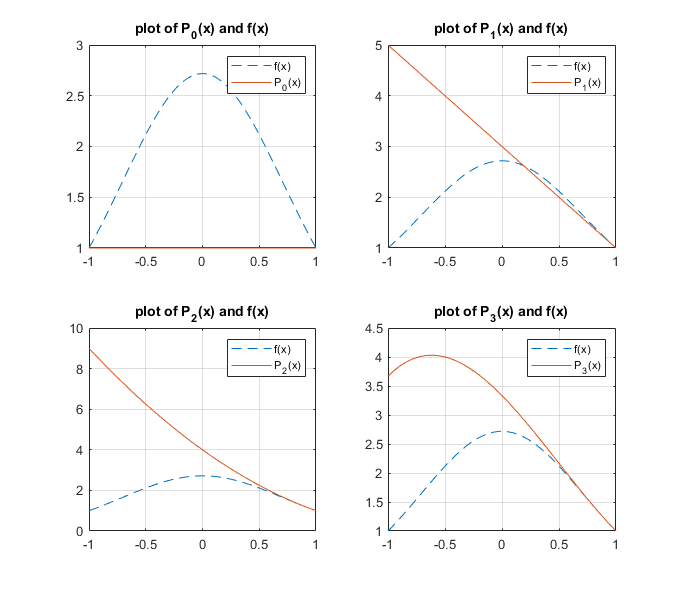
\includegraphics[width = \textwidth, Title = "Please Zoom"]{plotTaylor.png}







\end{exercise}

\end{document}